\documentclass{ctexart}
\usepackage{graphicx, hyperref}

\begin{document}
\title{可行性报告}
\author{马凯,金孜达,刘时,徐亦尧,李文睿}
\maketitle
\tableofcontents
\newpage

\section{可行性分析}
\subsection{理论依据}
\subsubsection{CAP定理}
CAP定理(CAP theorem),又被称作布鲁尔定理(Brewer's theorem),它指出对于一个分布式计算系统来说,不可能同时满足以下三点:
\begin{itemize}
    \item 一致性(Consistence) (等同于所有节点访问同一份最新的数据副本)
    \item 可用性(Availability)(每次请求都能获取到非错的响应——但是不保证获取的数据为最新数据)
    \item 分区容错性(Network partitioning(英语:Network partitioning)即使任意数量的消息被节点之间的网络丢弃(或延迟),系统仍继续运行(以实际效果而言,分区相当于对通信的时限要求。系统如果不能在时限内达成数据一致性,就意味着发生了分区的情况,必须就当前操作在C和A之间做出选择。)
\end{itemize}

根据定理,分布式系统只能满足三项中的两项而不可能满足全部三项。理解CAP理论的最简单方式是想象两个节点分处分区两侧。允许至少一个节点更新状态会导致数据不一致,即丧失了C性质。如果为了保证数据一致性,将分区一侧的节点设置为不可用,那么又丧失了A性质。除非两个节点可以互相通信,才能既保证C又保证A,这又会导致丧失P性质。

我们的项目抛弃了一致性(C),选择了可用性(A)和分区容错性(P)。

若设备离线,设备获取到的数据存储在本地,如果存储空间已满,系统就会抛弃旧的数据来接收新数据,向系统写入时永远不会报错,但由于旧数据被抛弃,从而失去了一致性。

\subsubsection{存储系统的性能指标}

存储系统有三个关键的性能衡量指标,分别为系统的读写速度、可靠性与耐久性(Durability)。下面分别说明

\begin{itemize}
    \item 读写速度:决定系统的带宽,常用单位时间读取/写入的数据量衡量,与存储系统的工作原理与结构设计相关。
    \item 可靠性:衡量系统损坏时保持数据不被破坏能力的指标:可靠性越强,系统就可以在受到越严重破坏的情况下恢复原有数据。常使用冗余存储来实现,通过建立数据镜像或存储校验位来实现恢复受损系统中数据的功能。
    \item 耐久性:衡量系统在异常断电后保留数据的能力。例如磁盘和闪存构成的存储系统一般具有高耐久性,因为这些介质的存储不依赖于电力。
\end{itemize}

这里需要提到的一点是,其实可靠性的定义不唯一,另一种定义为:可靠性是衡量系统保持正常工作能力的指标,常用MTBF(Mean Time Between Failure,平均故障间隔时间)来衡量。MTBF越长,系统在两次故障间正常工作时间的期望值约长。我们认为这种定义是对各种系统通用的,而先前的定义是存储系统所特有的,所以强调保持数据的定义。与前一种可靠性对应的还有一种可用性(Availability)的定义:衡量系统可用程度的指标,常用公式MTBF/(MTTR + MTBF)\footnote{MTTR: Mean Time To Repair,平均故障修复时间,与MTBF类似}衡量。

以上的每一种性能指标,都有对应的优化方法,例如读写速度可以通过RAID0来提高,可靠性可以通过RAID1来提高等。

(参考文献:\\
https://www.quora.com/Whats-the-difference-between-Reliability-Durability-and-Availability-for-data-storage-system, \\ https://en.wikipedia.org/wiki/Mean\_time\_between\_failures)

\subsubsection{加密传输}
用密码学能做什么
\begin{itemize}
	\item 保密性(Confidentiality)是一种服务,用于保持信息内容只有获得授权的人才能访问。该服务既包括保护在一段时间内在两点之间传输的所有用户数据,也包括保护分析过程中的传输。
	\item 完整性(Integrity)是一项服务,要求计算机系统资产和传输信息只能由授权用户进行修改。修改包括编写,更改,更改状态,删除,创建以及延迟或重新发送传输的消息。需要指出的是,整合与活动有关,因此它与检测而不是预防有关。更重要的是,可以提供或不提供恢复,第一选项是更具吸引力的替代方案。
	\item 认证(Authentication)是一种服务,关心的是确保消息的来源被正确识别。也就是说,应该通过渠道获得的信息可以在源头,起源日期,数据内容,发送时间等方面进行验证。由于这些原因,该服务被细分为两大类:实体验证和数据源验证。请注意,第二类认证隐式提供了数据整合度。
	\item 不可否认(Non-repudiation)是一种防止发送方和接收方拒绝先前承诺或行为的服务。
\end{itemize}

考虑到物联网设备中信息的传输可能被拦截,可能导致信息获取错误、信息泄露等后果,我们决定在信息的传输中使用加密手段,非对称加密较为安全,但消耗的资源较多,在资源严重限制的嵌入式设备上,信息全部使用非对称加密可能较为困难,因此我们决定使用非对称加密传输密钥,再用传输的密钥使用对称加密,这样即保证了安全性,也能在资源有限的嵌入式设备上尽可能的保持性能。

\paragraph{D-H密钥交换}
迪菲-赫尔曼密钥交换(英语:Diffie–Hellman key exchange,缩写为D-H) 是一种安全协议。它可以让双方在完全没有对方任何预先信息的条件下通过不安全信道创建起一个密钥。这个密钥可以在后续的通讯中作为对称密钥来加密通讯内容。

这个协议使用一个质数p的整数模n乘法群以及其原根g。
\begin{itemize}
	\item 爱丽丝与鲍伯协定使用$p=23$以及base $g=5$.
	\item 爱丽丝选择一个秘密整数$a=6$, 计算$A = g^a \bmod{p}$并发送给鲍伯。 $A = 5^6 \bmod{23} = 8$.
	\item 鲍伯选择一个秘密整数$b=15$, 计算$B = g^b \bmod{p}$并发送给爱丽丝。 $B = 5^{15} \bmod{23} = 19$.
	\item 爱丽丝计算$s = B^a \bmod{p}$,$19^6 \bmod{23} = 2$.
	\item 鲍伯计算$s = A^b \bmod{p}$,$8^{15} \bmod{23} = 2$.
\end{itemize}
爱丽丝和鲍伯最终都得到了同样的值,因为在模$p$下$g^{ab}和g^{ba}$ 相等。 注意$a, b$ 和 $g^{ab} = g^{ba} \bmod{p}$ 是秘密的。 其他所有的值 —$p, g$, $g^a \bmod{p}$, 以及 $g^b \bmod{p}$ 都可以在公共信道上传递。 一旦爱丽丝和鲍伯得出了公共秘密,他们就可以把它用作对称密钥,以进行双方的加密通讯,因为这个密钥只有他们才能得到。 当然,为了使这个例子变得安全,必须使用非常大的$a, b$ 以及 $p$, 否则可以实验所有$g^{ab} \bmod{23}$的可能取值(总共有最多22个这样的值, 就算a和b很大也无济于事)。 如果 $p$ 是一个至少 300 位的质数,并且$a$和$b$至少有100位长, 那么即使使用全人类所有的计算资源和当今最好的算法也不可能从$g, p$和$g^a \bmod{p}$ 中计算出 $a$。这个问题就是著名的离散对数问题。注意$g$则不需要很大, 并且在一般的实践中通常是2或者5。IETF RFC3526 文档中有几个常用的大素数可供使用。

D-H密钥交换较不安全,可以用中国剩余定理(CRT)破解,但如果取的数字较大,还是较为安全的,而且易于在资源较少的嵌入式设备上实现。

\paragraph{EDCH}
椭圆曲线迪菲-赫尔曼金钥交换(英语:Elliptic Curve Diffie–Hellman key Exchange,缩写为ECDH),一种匿名的密钥合意协议(Key-agreement protocol)。在这个协定下,双方通过迪菲-赫尔曼密钥交换演算法,利用由椭圆曲线加密建立的公钥与私钥对,在一个不安全的通道中,建立起安全的共有加密资料。这是迪菲-赫尔曼密钥交换的变种,采用椭圆曲线加密来加强安全性。

椭圆曲线密码学(英语:Elliptic curve cryptography,缩写为 ECC),一種建立公开密钥加密的演算法,基于椭圆曲线数学。

ECC的主要优势是在某些情况下它比其他的方法使用更小的密钥——比如RSA加密算法——提供相当的或更高等级的安全。ECC的另一个优势是可以定义群之间的双线性映射,基于Weil对或是Tate对;双线性映射已经在密码学中发现了大量的应用,例如基于身份的加密。不过一个缺点是加密和解密操作的实现比其他机制花费的时间长。

ECDH虽然很安全,但较为计算密集,在资源受限的嵌入式设备上实现可能很困难。

\paragraph{RSA加密}
RSA加密演算法是一种非对称加密演算法

对极大整数做因数分解的难度决定了RSA算法的可靠性。换言之,对一极大整数做因数分解愈困难,RSA算法愈可靠。假如有人找到一种快速因数分解的算法的话,那么用RSA加密的信息的可靠性就肯定会极度下降。但找到这样的算法的可能性是非常小的。今天只有短的RSA钥匙才可能被强力方式解破。到目前为止,世界上还没有任何可靠的攻击RSA算法的方式。只要其钥匙的长度足够长,用RSA加密的信息实际上是不能被解破的。

公钥与私钥的产生

假设Alice想要通过一个不可靠的媒体接收Bob的一条私人讯息。她可以用以下的方式来产生一个公钥和一个私钥:

\begin{itemize}
	\item 随意选择两个大的质数p和q,p不等于q,计算N=pq。
	\item 根据欧拉函数,求得$r=\varphi (N) = \varphi (p)\varphi (q)=(p-1)(q-1)$
	\item 选择一个小于r的整数e,使e与r互质。并求得e关于r的模反元素,命名为d(求d令${\displaystyle ed\equiv 1{\pmod{r}}}$)。模反元素存在,当且仅当e与r互质)
	\item 将p和q的记录销毁。
\end{itemize}

(N,e)是公钥,(N,d)是私钥。 Alice将她的公钥(N,e)传给Bob,而将她的私钥(N,d)藏起来。

\paragraph{加密消息}
${\displaystyle c\equiv n^{e}{\pmod {N}}}$
\paragraph{解密消息}
${\displaystyle c^d\equiv n{\pmod {N}}}$

RSA的算法实现也有些复杂,可能不适于在嵌入式系统实现。

总的来说,若想在嵌入式系统使用非对称加密算法加密传输的密钥,D-H加密可能是较好的选择。
\subsection{技术依据}
\subsubsection{RIOT OS}
本项目基于 RIOT 实现是可行的。下面给出主要依据。

\paragraph{架构}
RIOT 是微内核架构,整体高度模块化。这为本项目成员理解、修改操作系统代码创造了方便。

\begin{figure}
	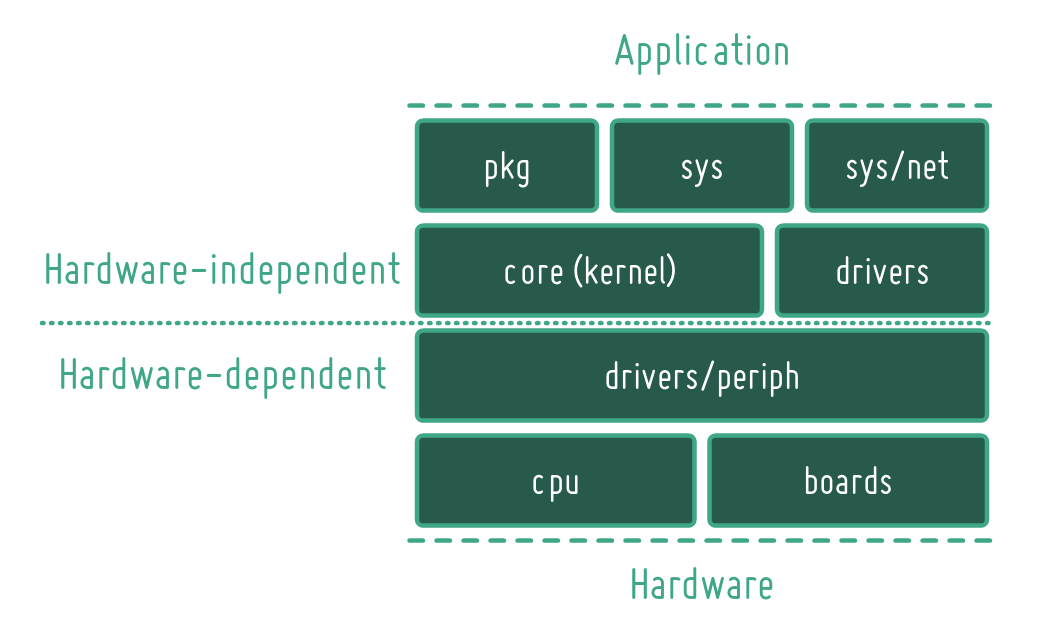
\includegraphics[width=\textwidth]{RIOT-Overview.png}
	\caption{RIOT OS 架构}
	\label{RIOT-Overview}
\end{figure}

\paragraph{资源占用}
RIOT 在极限情况下资源占用极低(见图 \ref{RIOT-Resource}),尽管不如 Tiny OS,但已经可以满足在苛刻的环境中使用。
这与本项目的目标使用场景极为匹配。

\begin{figure}
	\centering
	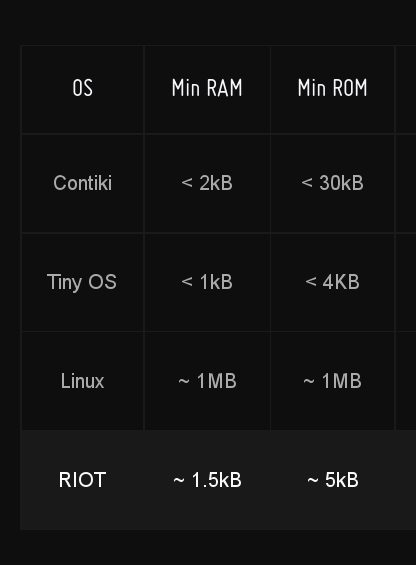
\includegraphics[scale=0.3]{RIOT-Resource.png}
	\caption{RIOT OS 资源占用}
	\label{RIOT-Resource}
\end{figure}


\paragraph{网络栈}
RIOT 提供了完整的网络栈,包括套接字接口和 IP、TCP、UDP 等协议的支持,这为本项目的网络功能实现提供了坚实的基础。RIOT 的模块化设计使得网络协议的替换也更加方便。

\paragraph{调度}
RIOT 调度的基本单位是线程,提供抢占式(半协作式)调度方式,且调度开销很低(不使
用周期性的时钟中断)。每个线程有一个 nice 值,值越大,优先级越低。当出现调度机会
时,优先级高的线程将总被执行。若优先级相同,则使用协作式调度策略,即通过
\verb|thread_yield| 交还 CPU 时间。

综上所述,RIOT 为本项目开展提供了极大方便,使得我们无需自己实现这些基础性功能,而是专注于项目本身的创新和设计。

\subsubsection{中心节点(server)的结构设计}

本项目的中心节点主要的任务是作为一个文件服务器(file server),存储由各端点分享的文件,并使之在所有端点可用。它本身不需要执行计算任务或对数据做处理,只要作为一个系统的数据中心即可。当某端点需要来自另一端点的文件时可以通过它获取到,而当用户访问系统时,可以在中心节点得到整理后的所有端点数据,这就是我们想让中心节点做的事情。

文件服务器的设计要考虑诸多因素,例如存储容量、访问速度、可恢复性、易管理性、安全性和预算等。除此之外,存储系统是文件服务器的重要部分,所以还要考虑存储系统的性能指标(读写性能、可靠性、耐久性等)。\footnote{这其中部分指标有重叠,例如服务器的可恢复性和存储系统的可靠性。}

在设计文件服务器时,可以参考NAS(Network-attached storage),两者的区别在于NAS一般是定制化的设备,且专门用于联网存储数据而没有更一般的计算功能。NAS的结构简单来说就是控制+存储,其中存储部分即一个存储系统,常用RAID;控制部分需要在设备上实现网络传输协议软件,可以有基于计算机、嵌入式设备和ASIC等多种实现。这三种实现的系统功耗和性能都由高到低排列,这里的性能主要反映在读写速度上。

我们初步的设想是实现基于计算机的文件服务器。这样做有两个好处:第一,PC作为中心节点的控制中枢使我们能够方便地访问中心节点,便于系统的测试与管理,让我们能聚焦于优化端点的存储与传输性能,免于花过多时间纠结在中心节点的访问上,这不是我们项目的关键所在;第二,PC的性能冗余使我们可以考虑为文件服务器增加更多功能,丰富项目的应用场景。事实上,实现数据在移动端的访问与管理,以及为文件服务器增加更多实用功能是本项目的两个重要的拓展方向。

(参考文献:https://en.wikipedia.org/wiki/Server\_(computing)\\
 https://en.wikipedia.org/wiki/File\_server\\ https://en.wikipedia.org/wiki/Communications\_server\\ https://en.wikipedia.org/wiki/Network-attached\_storage)

\section{概要设计报告}

\subsection{简介}
本节介绍整个系统的总体结构。

本项目不仅仅是文件系统,而是与之相关的一整套配套设施。包括两大组件:
\begin{enumerate}
	\item 适用于物联网设备的文件系统;
	\item 中心服务程序。
\end{enumerate}
在这个系统中,运行文件系统的设备称为\textbf{客户端}(client),运行中心服务程序的计算机称为\textbf{服务器}(server)。
整个系统的网络形态是以服务器为中心的星形结构(图 \ref{design-net-topo})。在这里,一条边并不意味着实际的网络连接(例如 TCP 连接),
而是代表一种逻辑从属关系(详见小节 \ref{design-network})。下文中把客户端和服务器的这种情形叫做逻辑连接。

\begin{figure}
	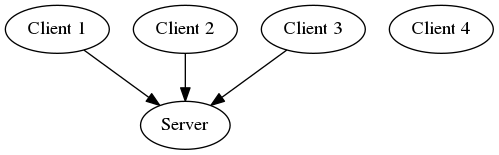
\includegraphics[width=\textwidth]{design-net-topo.png}
	\caption{网络拓扑示意图}
	\label{design-net-topo}
\end{figure}

作为一个文件系统,每个客户端也可以独立工作(如图 \ref{design-net-topo} 中的 Client 4)。

每个客户端可以按需选择连接不同的服务器。但出于安全性考虑,设备和服务器需双方验证通过并建立加密传输通道后方可建立逻辑连接(详见小节 \ref{design-security})。

通常情况下,每个客户端的文件系统可以存在以下资源:
\begin{enumerate}
	\item 一般文件(详见小节 \ref{design-fs});
	\item 流数据管道(详见小节 \ref{design-stream});
	\item 消息管道(详见小节 \ref{design-message})。
\end{enumerate}
其中,\textbf{管道}指网络资源在本地文件系统的映射,但占据本地存储空间。
对客户端应用程序来说,以上三种资源是使用统一的命名空间进行访问和操作,即这些资源均可看作文件。
但是,流数据管道或只允许写操作、或只允许读操作,而请求管道多次读取数据可能不一样。

每次打开管道,都必须首先与服务器建立逻辑连接。第二次建立打开管道时,可以复用此前的逻辑连接。从服务器发送来的数据将自动保存在本地存储空间中,直到用户程序读取而消耗之。向可写管道中写入数据,写入数据则将自动被发送到服务器。
\begin{enumerate}
	\item 当数据写入可写流数据管道时,这部分数据将被原样发送到服务器。
	\item 当数据写入消息管道时,这部分数据将以 MQTT 消息的形式原子地发送到服务器。
\end{enumerate}
若网络断开或拥堵,将在本地的存储空间中进行临时存储,以免数据丢失。若缓冲区已满,则按用户指定的替换策略丢弃一部分数据。

\subsection{文件系统设计}
\label{design-fs}
本项目的基础是文件系统,设计主要取自 LittleFS,但删除了目录,因为目录在本项目目
标使用场景中用处不大,反而大大复杂化了文件系统的设计。

\subsubsection{元数据}
\begin{verbatim}
struct metadata {
  char rev;
  char checksum;
  char file_type;
  char storage_type;
  void *ptr;
  long length;
  void *next;
  char filename[MAX_FILENAME];
  char info[MAX_BLOCK - MAX_FILENAME - OTHER_FIELDS_LEN];
};
\end{verbatim}

\begin{enumerate}
\item rev 是元数据块的更新版本。
\item checksum 是元数据块的校验和,用于检测异常情况。
\item file\_type 是文件类型,可取 F(一半文件) / WS(可写流) / RS(可读流) / MQ(消
  息管道)三类。
\item storage\_type 是存储的类型,可取前向链表、后向链表和连续存储。
\item ptr 是指向数据块的指针。若为前向链表,指向头节点;若为后向链表,指向尾节点;
  若为连续存储,指向首字节。
\item length 是文件大小,或缓冲区占用大小。
\item next 是指向下一个元数据的指针。
\item info 是用于管道的额外信息。
\end{enumerate}

在搜寻文件时,在元数据构成的链表上依次查找,直到找到匹配的文件。

每个元数据占用连续两块,每次修改时修改版本最低的那个,从而在意外情况下可以保证文
件旧数据仍能读出。

\subsubsection{文件数据的存储}

\begin{verbatim}
struct fwd_block {
  struct fwd_block *next;
  long size;
  char data[MAX_BLOCK - OTHER_FIELDS_LEN];
};

struct back_block {
  struct back_block *prev;
  long size;
  char data[MAX_BLOCK - OTHER_FIELDS_LEN];
};

struct contiguous {
  long len;
  char *buf;
};
\end{verbatim}

每次修改文件数据时,首先找到空闲块将修改过的数据写入其中,然后原子地更新元数据。
这样可以保证无论发生什么,总有一份可用的数据。

默认情况下,文件使用 fwd\_block,管道缓冲区使用连续存储。

fwd\_block 和 back\_block 分配新块时,总是从前向后扫描,而连续存储从后向前扫描。

\subsection{应用程序编程接口}
\label{design-api}
本项目的目标是提供一个接近标准 POSIX 文件 IO 的接口,但明确放弃了诸如权限控制等功能,这在嵌入式环境中意义不大。
由于本项目不支持目录,因此 \verb|/| 也可以用于文件名。

本项目提供以下接口:
\begin{enumerate}
	\item \verb|int link(const char *addr, int flags);|\\
	用于建立逻辑连接。返回逻辑连接 ID。
	\item \verb|int open(const char *filename, int flags);|\\
	用于打开文件或管道。打开管道时,使用最近一次的逻辑连接。
	\item \verb|int close(int fd_or_link);|\\
	用于关闭文件、管道或逻辑连接。一旦逻辑连接被关闭,与之相关的所有管道也将失效。
	\item \verb|ssize_t read(int fd, void *buf, size_t count);|\\
	用于从管道或文件中读取数据。
	\item \verb|ssize_t write(int fd, const void *buf, size_t count);|\\
	用于写文件或通过流数据管道传输数据。
\end{enumerate}

一个简单的视频监控示例程序如下:
\begin{verbatim}
int lnk = link("192.168.1.1:1234", L_SECRET);
int stream = open("video", O_WRS, SD_CARD_SIZE / 2); /* O_WRS 意为打开可写流 */
while (true) {
  size_t len;
  void *vbuf = getvideo(&len);
  write(stream, vbuf, len);
}
\end{verbatim}
该程序通过无限循环将捕获的视频数据源源不断地发送到服务器,并且无需担心数据传输的安全性和网络环境的稳定性。

\subsection{网络}
\label{design-network}
物联网设备普遍搭载有网络设备,通常都有 IP 地址,但为了安全性和更普遍的使用场景,本项目的网络环境要求仅仅为客户端与服务器之间可以建立连接。
设备与设备间的通讯将通过服务器中转。

本项目采用 TCP 和 UDP 协议。由于 UDP 是无状态的,不要求实际存在连接,因此服务器与客户端的连接关系称为逻辑连接。

当客户端与服务器建立逻辑连接时,首先建立不安全通信信道,随后进行密钥交换,这为接下来的加密通信建立了基础(详见小节 \ref{design-security})。
此时,服务端为该 IP 地址分配 ID,并记录在客户端列表上,直到该客户端下线时解除 IP 和 ID 之间的关系。

当客户端发起网络请求时,每次请求的数据(即流数据管道的一次 \verb|write|)将一并全部发向服务器,但并不处理流数据管道发送失败或部分发送失败
的情形。若消息管道发送失败,则重试发送整体,直到数据发送成功。

当网络操作失败时,将认为网络环境不稳定或网络已断开,因此断开一切连接。此时,一切写入操作将自动切换到本地缓冲区。后台以指定频率尝试重连,
一旦重连成功,则认为网络环境恢复正常,重新将本地缓冲区数据发送到服务器。此时若网络操作失败,则重新断开并继续尝试重连。

当服务器向客户端发送数据时,该数据首先保存在本地缓冲区。数据被 \verb|read| 则认为被消耗,这部分存储将被清除掉。

\subsection{网络资源映射}
网络资源的映射通过管道实现。本节详述管道的设计。

\subsubsection{流数据}
\label{design-stream}
流数据指能容忍一部分数据缺失的二进制流,如视频流、音频流等。

本项目中,流数据管道分为两种:
\begin{enumerate}
	\item 可读流数据管道:从服务器读取流数据;
	\item 可写流数据管道:向服务器传送流数据。
\end{enumerate}

当数据从服务器到达客户端时,这些数据被缓存在本地存储中。若缓冲区已满,则按替换策略(详见小节 \ref{design-replace})丢弃数据。

当数据从客户端发往服务器时,若数据成功发送,则不在本地缓存;若数据发送失败,则在本地进行缓存,从而为将来的重新发送做准备。若缓冲区已满,
则按替换策略丢弃一定数据,若不丢弃新数据,则丢弃旧数据直到有足够的空间存储新数据。这里直接丢弃整个块,而不在字节层面上丢弃,从而提高效率。
因此,流数据管道的写操作将永远不会失败。

由于流数据是以字节为单位的,故所有操作本身已经是原子的了,无需进一步设计。

\subsubsection{消息管道}
\label{design-message}
本项目将消息集成到文件系统中。消息的传输通道被称作消息管道。消息管道中的每个请求的发送和接收均是原子的,即每个消息要么不存在,要么必是
完整的。这在网络不稳定的环境中有一定应用价值。

消息管道的实现与数据流管道类似,区别是每次替换数据时依次替换掉已有消息,直到有足够空间容纳当前数据。正在被发送的块被标记为锁定,即无法被替换,避免不完整数据被发出。

\subsubsection{替换策略}
\label{design-replace}
本项目中本地存储常常被用作缓冲区使用,而在离线状态下,缓冲区很快就会填满,因此有必要提供替换策略。

替换在管道的缓冲过程中发生。不同管道可以有不同的替换策略。

本项目预设提供三种替换策略:
\begin{itemize}
	\item 丢弃:直接丢弃新数据,这种策略简单粗暴,但在部分情况下仍有实用价值,如在资源极为有限的情况下无法支持其他替换策略,而该策略已经可以减少数据损失;
	\item FIFO:丢弃最老的数据,这种策略适用于新数据优于老数据的场景,如温度计读取当前气温;
	\item 优先队列:丢弃优先级最低的数据(当所有数据优先级均一样时,使用其他替换策略),这种策略适用于数据优先级不定的场景,如传感器对数据采样,出现特定模式的数据优先级更高。
\end{itemize}
用户应该可以提供自己的替换策略。由于替换的发生必在管道被打开时,则在打开管道时提供一个自定义的替换函数即可实现。

由于流数据不存在结构,因此不能使用优先队列替换策略。

\subsection{安全性}
\label{design-security}
由于物联网设备可能暴露在开放环境中,这就使得数据的安全性受到威胁。本项目为此设计了安全传输策略。

每个设备可以根据需要附带一个信任服务器的公钥,在建立逻辑连接的过程中,客户端随机选定一个密钥并用公钥加密后送往服务器,
随后与服务器之间的所有网络流量均用此密钥对称加密。

由于对称加密对性能的影响很小,该方案一定程度上可以提供系统安全性。这个加密方案仍需要进一步的实验。

\subsection{调度策略}
鉴于本项目实现平台(实时操作系统)的特殊性,有必要考虑本项目为应用程序带来的开销,特别是网络相关功能。

RIOT 调度的基本单位是线程,每个应用程序包含至少两个线程 \verb|main| 和
\verb|idle|。每个线程都有 nice 值,高 nice 值的线程可以被低 nice 值的线程抢占执
行机会。

本项目虽然使用了大量网络功能,但仍要避免频繁切换造成的开销,也要避免不切换造成线
程饿死。为此,本项目的网络系统并不作为单独的一个线程,而是做进系统内核,实现更灵
活的调度策略。
\begin{enumerate}
\item 在程序进行 IO 操作时,向设备发出请求后立刻 yield;
\item 当网络数据到达时,中断处理程序立刻将数据保存到内存和缓冲区,并向线程发送消
  息通知数据到达。
\end{enumerate}
考虑到 RIOT 调度模型,这在普通的线程模型下很难做到。

综上所述,本项目将作为 RIOT module 或 kernel patch 发布。

\end{document}
